% Paquets généraux
\documentclass[a4paper,12pt,titlepage]{article}
\usepackage[T1]{fontenc}
\usepackage[utf8]{inputenc}
\usepackage[french]{babel}
\usepackage[gen]{eurosym}
%\usepackage[dvips]{graphicx}
\usepackage{fancyhdr}
\usepackage{pdfpages} 
\usepackage{multido}
\usepackage{hyperref}
%\usepackage{textcomp}
%\usepackage{aeguill}
\usepackage{schemabloc}
\usepackage[bitstream-charter]{mathdesign}

\newcommand{\id}{54}
\newcommand{\nom}{Liaisons mécaniques}
\newcommand{\sequence}{04}
\newcommand{\num}{01}
\newcommand{\type}{TP}
\newcommand{\descrip}{Modélisation d'un solide. Comportement des liaisons mécaniques. Modéliser les mécanismes du laboratoire par un schéma cinématique, paramétré.}
\newcommand{\competences}{A3-C4: Analyse d'architecture et de comportement \\ &  Mod1-C1: Isolement d'un solide ou d'un système de solides \\ &  Mod2-C10-1: Modèle de solide indéformable \\ &  Mod2-C11: Modélisation géométrique et cinématique des mouvements entre solides indéformables \\ &  Mod2-C12: Modélisation cinématique des liaisons entre solides \\ &  Mod2-C15: Modélisation des actions mécaniques \\ &  Rés-C6: Utilisation d'un solveur ou d'un logiciel multi physique \\ &  Com1-C1: Différents descripteurs introduits dans le programme \\ &  Com2-C4: Outils de communication}
\newcommand{\nbcomp}{9}
\newcommand{\systemes}{Plateforme Stewart}
\newcommand{\systemessansaccent}{Plateforme Stewart}
\newcommand{\ilot}{2}
\newcommand{\ilotstr}{02}
\newcommand{\dossierilot}{\detokenize{Ilot_02 Plateforme Stewart}}
\newcommand{\imageun}{Plateforme}

\newcommand{\urlsysteme}{\href{https://www.costadoat.fr/systeme/57}{Ressources système}}
\newcommand{\matlabsimscape}{\href{https://github.com/Costadoat/Sciences-Ingenieur/raw/master/Systemes/Plateforme Stewart/Plateforme_Stewart_Simscape.zip}{Modèle Simscape}}
\newcommand{\solidworks}{\href{https://github.com/Costadoat/Sciences-Ingenieur/raw/master/Systemes/Plateforme Stewart/Plateforme_Stewart_Solidworks.zip}{Modèle Solidworks}}
\newcommand{\edrawings}{\href{https://github.com/Costadoat/Sciences-Ingenieur/raw/master/Systemes/Plateforme Stewart/Plateforme_Stewart.EASM}{Modèle eDrawings}}
\newcommand{\test}{Stewart_param1}
\newcommand{\testi}{Stewart_param2}
\newcommand{\testii}{Stewart_param3}
\newcommand{\testiii}{Stewart_param4}
\newcommand{\testiiii}{Stewart_euler}

\newcommand{\auteurun}{Renaud Costadoat}
\newcommand{\auteurdeux}{Françoise Puig}
\newcommand{\institute}{Lycée Dorian}


\usepackage{color}
\usepackage{xcolor}
\usepackage{colortbl}
\usepackage{helvet}
\renewcommand{\familydefault}{\sfdefault}
\usepackage{amsfonts}
\usepackage{amsmath}
%\usepackage{xspace}
\usepackage{varioref}
\usepackage{tabularx}
%\usepackage{floatflt}
\usepackage{graphics}
\usepackage{wrapfig}
\usepackage{textcomp}
\usepackage{tikz}
\usepackage{wrapfig}
\usepackage{gensymb}
\usepackage[european]{circuitikz}
\usetikzlibrary{babel}
\usepackage{ifthen}
\usepackage{cancel}
\usepackage{etoolbox}
\usepackage{multirow}
%\usepackage{boxedminipage}
\definecolor{gris25}{gray}{0.75}
\definecolor{bleu}{RGB}{18,33,98}
\definecolor{bleuf}{RGB}{42,94,171}
\definecolor{bleuc}{RGB}{231,239,247}
\definecolor{rougef}{RGB}{185,18,27}
\definecolor{rougec}{RGB}{255,188,204}%255,230,231
\definecolor{vertf}{RGB}{103,126,82}
\definecolor{vertc}{RGB}{220,255,191}
\definecolor{forestgreen}{rgb}{0.13,0.54,0.13}
\definecolor{blcr}{rgb}{0.59,0.69,0.84}
\definecolor{blfr}{rgb}{0.32,0.51,0.75}
\definecolor{orfr}{rgb}{0.90,0.42,0.15}
\definecolor{orcr}{rgb}{0.90,0.65,0.50}
\definecolor{orangef}{rgb}{0.659,0.269,0.072}
\definecolor{orange}{rgb}{0.58,0.35,0.063}
\definecolor{orangec}{rgb}{0.43,0.32,0.25}
\definecolor{rcorrect}{rgb}{0.6,0,0}
\definecolor{sequence}{rgb}{0.75,0.75,0.75}
\definecolor{competences}{rgb}{0.61,0.73,0.35}
\definecolor{grisf}{HTML}{222222}
\definecolor{grisc}{HTML}{636363}
\definecolor{normal}{HTML}{4087c4}
\definecolor{info}{HTML}{5bc0de}
\definecolor{success}{RGB}{92,184,92}
\definecolor{warning}{RGB}{240,173,78}
\definecolor{danger}{RGB}{217,83,79}
\hypersetup{                    % parametrage des hyperliens
    colorlinks=true,                % colorise les liens
    breaklinks=true,                % permet les retours à la ligne pour les liens trop longs
    urlcolor= blfr,                 % couleur des hyperliens
    linkcolor= orange,                % couleur des liens internes aux documents (index, figures, tableaux, equations,...)
    citecolor= forestgreen                % couleur des liens vers les references bibliographiques
    }

% Mise en page
\pagestyle{fancy}

\setlength{\hoffset}{-18pt}

\setlength{\oddsidemargin}{0pt} 	% Marge gauche sur pages impaires
\setlength{\evensidemargin}{0pt} 	% Marge gauche sur pages paires
\setlength{\marginparwidth}{00pt} 	% Largeur de note dans la marge
\setlength{\headwidth}{481pt} 	 	% Largeur de la zone de tête (17cm)
\setlength{\textwidth}{481pt} 	 	% Largeur de la zone de texte (17cm)
\setlength{\voffset}{-18pt} 		% Bon pour DOS
\setlength{\marginparsep}{7pt}	 	% Séparation de la marge
\setlength{\topmargin}{-30pt} 		% Pas de marge en haut
\setlength{\headheight}{35pt} 		% Haut de page
\setlength{\headsep}{20pt} 		% Entre le haut de page et le texte
\setlength{\footskip}{30pt} 		% Bas de page + séparation
\setlength{\textheight}{700pt} 		% Hauteur de l'icone zone de texte (25cm)
\setlength\fboxrule{1 pt}
\renewcommand{\baselinestretch}{1}
\setcounter{tocdepth}{1}
\newcommand{\cadre}[2]
{\fbox{
  \begin{minipage}{#1\linewidth}
   \begin{center}
    #2\\
   \end{center}
  \end{minipage}
 }
}

\newcounter{num_quest} \setcounter{num_quest}{0}
\newcounter{num_rep} \setcounter{num_rep}{0}
\newcounter{num_cor} \setcounter{num_cor}{0}

\newcommand{\question}[1]{\refstepcounter{num_quest}\par
~\ \\ \parbox[t][][t]{0.15\linewidth}{\textbf{Question \arabic{num_quest}}}\parbox[t][][t]{0.93\linewidth}{#1}\par
}


\newcommand{\reponse}[1]
{\refstepcounter{num_rep}
\noindent
\rule{\linewidth}{.5pt}
\textbf{Question \arabic{num_rep}:}
\multido{\i=1+1}{#1}{~\ \\}
}

\newcommand{\cor}
{\refstepcounter{num_cor}
\noindent
\rule{\linewidth}{.5pt}
\textbf{Question \arabic{num_cor}:} \\
}

\newcommand{\titre}[1]
{\begin{center}
\cadre{0.8}{\huge #1} 
\end{center}
}


% En tête et pied de page
\fancypagestyle{normal}{%
  \fancyhf{}
\lhead{\nom}
\rhead{
\includegraphics[width=2cm]{../../img/logo}\hspace{2pt}}
\ifdef{\auteurdeux}{\lfoot{\auteurun,\auteurdeux}}{\lfoot{\auteurun}}
\cfoot{Page \thepage}}

\fancypagestyle{correction}{%
  \fancyhf{}
  \lhead{\colorbox{danger}{\begin{minipage}{0.65\paperwidth} \textcolor{white}{\textbf{Correction}} \end{minipage}} }
  \rhead{
\includegraphics[width=2cm]{../../img/logo}}
  \ifdef{\auteurdeux}{\lfoot{\auteurun,\auteurdeux}}{\lfoot{\auteurun}}
  \rfoot{\colorbox{danger}{\begin{minipage}{0.5\paperwidth} \begin{flushright}\textcolor{white}{\textbf{Correction}}\end{flushright} \end{minipage}} }}

\renewcommand{\footrulewidth}{0.4pt}

\usepackage{eso-pic}
\newcommand{\BackgroundPic}{%
\put(0,0){%
\parbox[b][\paperheight]{\paperwidth}{%
\vfill
\begin{center}
\hspace{0.5cm}\vspace{0.5cm}

\includegraphics[width=\paperwidth,height=\paperheight,%
keepaspectratio]{../../img/fond3}%
\end{center}
\vfill
}}}

\newcommand{\BackgroundPicdeux}{%
\put(25,-30){%
\parbox[b][\paperheight]{\paperwidth}{%
\vfill
\begin{center}
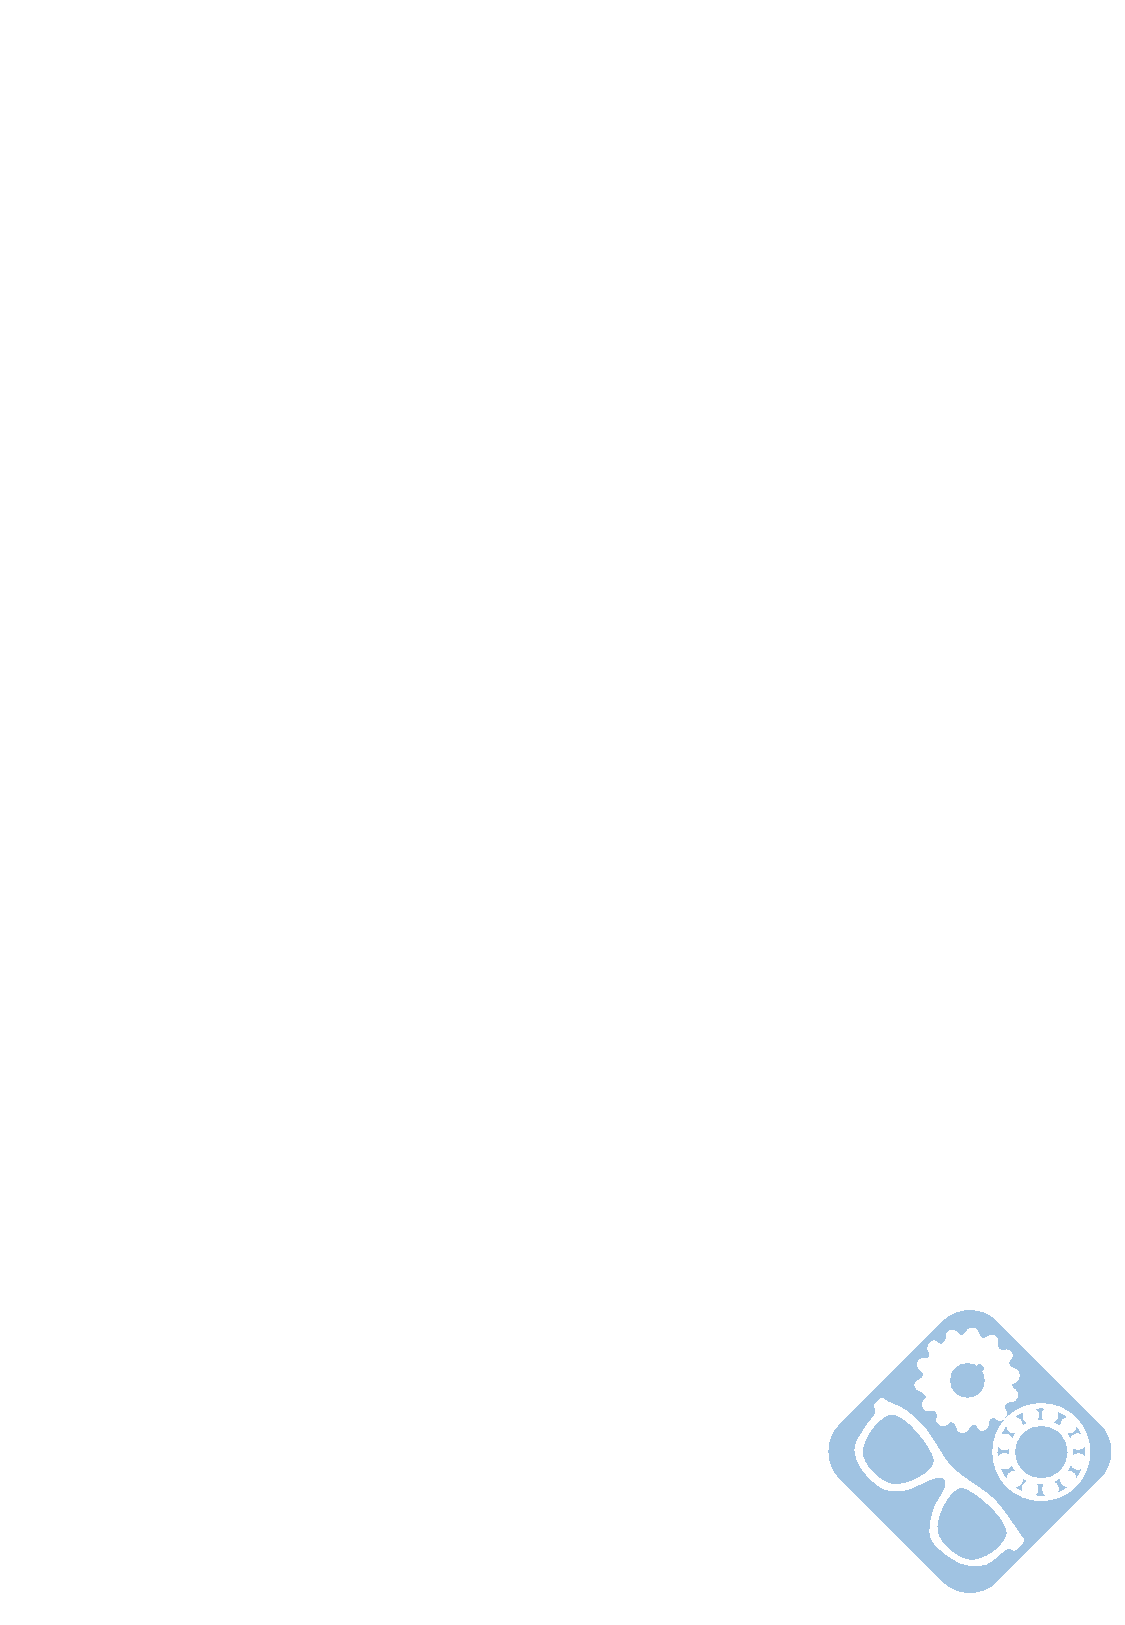
\includegraphics[width=\paperwidth,height=\paperheight,%
keepaspectratio]{../../img/fond4}%
\end{center}
\vfill
}}}

\begin{document}

\pagestyle{empty}

\vspace*{-3\baselineskip}

\AddToShipoutPicture*{\BackgroundPic}

\ifdef{\auteurdeux}{\begin{tabular}{>{\columncolor{gray!00}}m{.3\linewidth} m{.3\linewidth} >{\columncolor{gray!00}}m{.3\linewidth}}
Séquence : \sequence &  \multirow{3}{*}{\hspace{1cm}
\includegraphics[height=1.5cm]{../../img/logo}} &  \begin{flushright} \multirow{4}{*}{\hspace{1cm}
\includegraphics[height=4cm]{img/qrcode}}\end{flushright}\\
Document : \type\num \\
 \institute \\
 \auteurun\\
 \auteurdeux
\end{tabular}}{\begin{tabular}{>{\columncolor{gray!00}}m{.3\linewidth} m{.3\linewidth} >{\columncolor{gray!00}}m{.3\linewidth}}
Séquence : \sequence &  \multirow{3}{*}{\hspace{1cm}
\includegraphics[height=1.5cm]{../../img/logo}} &  \begin{flushright} \multirow{4}{*}{\hspace{1cm}
\includegraphics[height=4cm]{img/qrcode}}\end{flushright}\\
Document : \type\num \\
 \institute \\
 \auteurun
\end{tabular}}

\vspace{1cm}

\ifdef{\prive}{\begin{center}\colorbox{danger}{\Huge{Avec Correction}}\end{center}}{}

\begin{center}\huge{\nom}\end{center}

\vspace{2cm}

\ifdef{\imagedeux}{\begin{minipage}{0.49\linewidth}}{}
\begin{center}\includegraphics[height=5cm]{/home/renaud/Documents/Renaud/GitHub/django_education/systemes/\imageun}\end{center}
\ifdef{\imagedeux}{\end{minipage}\hfill
\begin{minipage}{0.49\linewidth}
\begin{center}\includegraphics[height=5cm]{/home/renaud/Documents/Renaud/GitHub/django_education/systemes/\imagedeux}\end{center}
\end{minipage}}{}

\vspace{5cm}


\begin{tabular}{p{.15\linewidth} >{\columncolor{white}}p{.8\linewidth}}
    \rowcolor{gray!20}
    Référence & S\sequence\ - \type\num \\
    Compétences & \competences \\
 	\rowcolor{gray!20}
    Description & \descrip \\
    Système & \systemes
  \end{tabular}

\newpage

\AddToShipoutPicture{\BackgroundPicdeux}

\pagestyle{normal}

\section{Mandrin à serrage pneumatique}

\begin{figure}[!h]
  \begin{minipage}{0.35\linewidth}
  \centering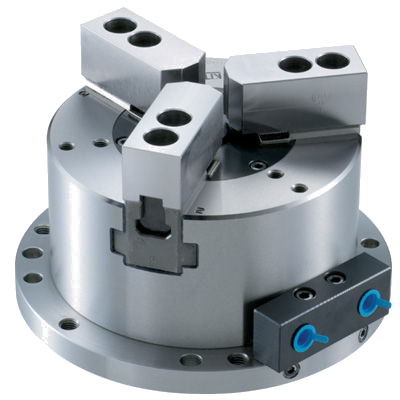
\includegraphics[width=0.7\linewidth]{img/mandrin}
  \end{minipage}
  \hfill
  \begin{minipage}{0.60\linewidth}
Le mandrin est un système mécanique fixée au bout de l'arbre d'une machine des mors vers le centre pour un serrage extérieur de la pièce, ou vers l'extérieur pour un serrage intérieur de la pièce. 

Le système étudié est un mandrin expansif (serrage par l'intérieur) à commande pneumatique. 
  \end{minipage}
\end{figure}

\begin{figure}[!h]
  \begin{minipage}{0.48\linewidth}
  \centering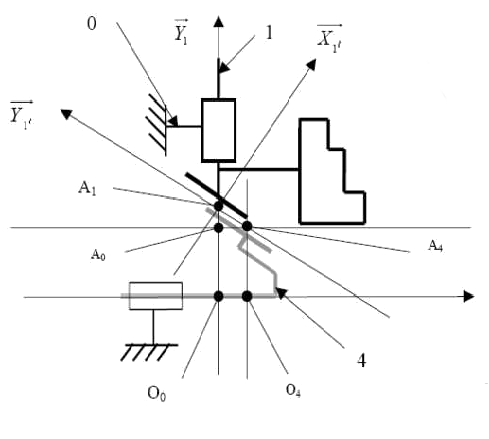
\includegraphics[width=.9\linewidth]{img/mandrin_cin.png}
  \end{minipage}
  \hfill
  \begin{minipage}{0.48\linewidth}
Cette partie va consister à déterminer les efforts qui s'exercent sur la pièce 5 dans l'étude afin de vérifier la donnée fournie par le fabricant du mandrin qui donne une action de serrage de 500 daN sous une pression de fonctionnement de 30 bars. \\
$\overrightarrow{O_0A_i}=e.\overrightarrow{Y_i}$ et $\alpha=30\degree$.
 \end{minipage}
\end{figure}

Pour simplifier le problème, on fera les hypothèses suivantes : 
\begin{itemize}
 \item Le poids des pièces sera négligé devant les actions mécaniques de liaisons. 
 \item Pas de frottement au niveau des contacts des liaisons au sein du mandrin. 
 \item Répartition uniforme des pressions de contact entre les différents solides et la pression du fluide sur la face du piston. Le piston est représenté à la fin du sujet.
\end{itemize}

\paragraph{Question 1:} Déterminer le torseur $\left\{T_f\right\}$ d'action du fluide sur le piston 4 au point $O_0$ dans la base $(\overrightarrow{x_0},\overrightarrow{y_0},\overrightarrow{z_0})$.

Pour l'application numérique, soit D le diamètre extérieur du piston et d le diamètre intérieur du piston : D = 157 mm, d = 45mm. 

~\

\textbf{Modélisation de l'action mécanique des 3 mors sur le piston 4}

~\

  \begin{minipage}{0.35\linewidth}
  \centering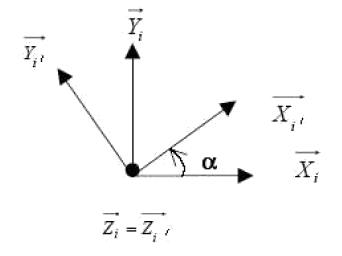
\includegraphics[height=4cm]{img/param_man_2_2.png}
  \end{minipage}  \hfill
  \begin{minipage}{0.6\linewidth}
	\paragraph{Question 2:} Écrire le torseur d'actions mécaniques du mors i sur le piston 4 en $O_0$ dans la base $R_i$.\\
	Rappel: $\overrightarrow{O_0A_i}=e.\overrightarrow{Y_i}$.
  \end{minipage}

\newpage

Paramétrage des repères lies aux mors 1, 2, et 3 

\begin{figure}[!h]
  \begin{minipage}{0.48\linewidth}
  \centering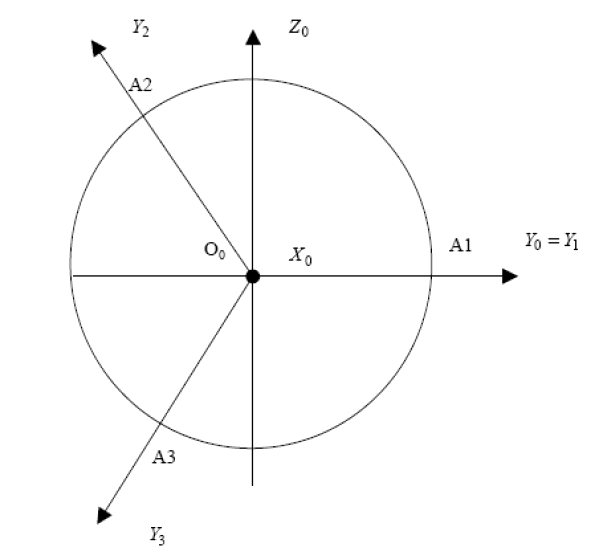
\includegraphics[height=4cm]{img/param_man_1.png}
  \end{minipage}
  \begin{minipage}{0.48\linewidth}
  \centering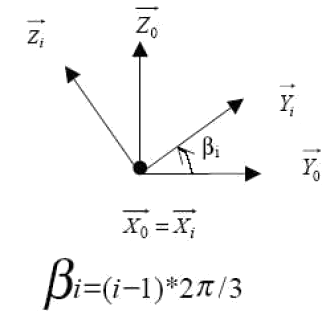
\includegraphics[height=4cm]{img/param_man_2_1.png}
  \end{minipage}  \hfill
\end{figure}

On donne (ci-dessus) le paramétrage des 3 repères lies au mors 1,2 et 3. On supposera que les actions mécaniques des 3 mors sur le piston 4 sont identiques. 

\paragraph{Question 3:} Montrer que le torseur des actions mécaniques de l'ensemble des 3 mors sur le piston 4 au point O0 et dans la base $(\overrightarrow{x_0},\overrightarrow{y_0},\overrightarrow{z_0})$, en fonction des composantes du torseur d'action du mors 1 sur le piston 4 est de la forme : 

$\left\{T_{\sum Mors \rightarrow S_4}\right\}=\left\{
  \begin{array}{c c}
  X_{\sum Mors \rightarrow S_4} & L_{\sum Mors \rightarrow S_4} \\
  0 & 0 \\
  0 & 0
  \end{array}\right\}_{O,R_0}$

\paragraph{Question 4:} Donner les valeurs de $X_{\sum Mors \rightarrow S_4}$ et $L_{\sum Mors \rightarrow S_4}$

~\

\textbf{Détermination de l'action du corps 0 sur le piston 4}

\paragraph{Question 5:} Écrire le torseur d'action mécanique de liaison entre le corps du mandrin 0 et le piston 4 en $O_0$ dans la base $(\overrightarrow{x_0},\overrightarrow{y_0},\overrightarrow{z_0})$. 
 
\paragraph{Question 6:} Écrire les 6 équations scalaires traduisant l'équilibre du piston 4. 

\paragraph{Question 7:} En déduire l'action du corps 0 sur le piston 4 et commenter le résultat. 

\paragraph{Question 8:} Déterminer la valeur de $M_{14}$ et l'expression de $X_{14}$ fonction de $X_f$ et de $\alpha$.

~\

\textbf{Détermination de l'action de serrage de la pièce 5 sur le mors 1}

\paragraph{Question 9:} Écrire le torseur d'action mécanique de liaison entre le corps 0 et le mors 1 en $O_0$ dans la base $(\overrightarrow{x_0},\overrightarrow{y_0},\overrightarrow{z_0})$. 

On donne le torseur d'action mécanique de la pièce 5 sur le mors 1 au point de contact P (un coefficient de frottement $f=0.3$ sera à prendre en compte) : 

$\left\{T_{5 \rightarrow 1}\right\}=\left\{
  \begin{array}{c c}
  X_{51} & 0 \\
  Y_{51} & 0 \\
  Z_{51} & 0
  \end{array}\right\}_{p,R_1}$, avec $\overrightarrow{O_0P}=R.\overrightarrow{Y_1}$.

\paragraph{Question 10:} Écrire les 6 équations scalaires traduisant l'équilibre du mors 1. 

\paragraph{Question 11:} Déterminer $Y_{51}$ en fonction de $X_f$ et $\alpha$. 

\paragraph{Question 12:} Compte tenu des hypothèses, commenter le résultat obtenu et vérifier la capacité de serrage du mandrin.

\paragraph{Question 13:} En déduire la valeur de la composante $Z_{5 \rightarrow 1}$. Déterminer alors la valeur du couple sur $\overrightarrow{x}$ transmis par le mandrin. Le diamètre de serrage est $R=10mm$.

\begin{figure}[!h]
  \begin{minipage}{0.48\linewidth}
  \centering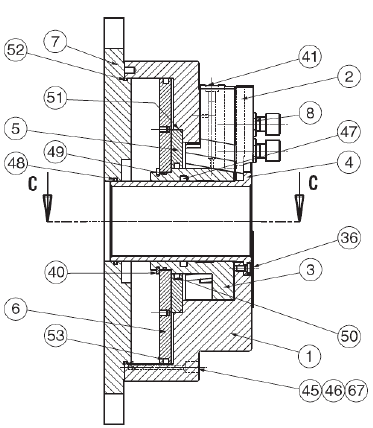
\includegraphics[width=.9\linewidth]{img/mandrin_dessin_1}
  \end{minipage}
  \hfill
  \begin{minipage}{0.48\linewidth}
  \centering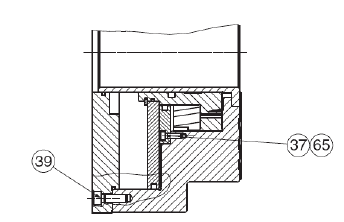
\includegraphics[width=.9\linewidth]{img/mandrin_dessin_2}
 \end{minipage}
\end{figure}

\newpage

\section{Serre joint}

\begin{figure}[!h]
  \begin{minipage}{0.35\linewidth}
  \centering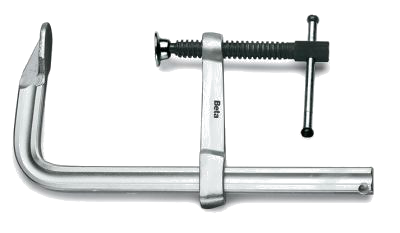
\includegraphics[width=\linewidth]{img/serre-joint}
  \end{minipage}
  \hfill
  \begin{minipage}{0.60\linewidth}
Un serre-joint est un outil de maçon ou de menuisier. Il permet de serrer et de maintenir différentes pièces en contact entre elles.

Le serre-joint utilisé en maçonnerie est constitué de deux pièces métalliques, la plus courte coulissant sur la partie plus longue de l'autre pour s'adapter à l'épaisseur à soumettre à la contrainte. Il est employé dans la réalisation de coffrage. 
  \end{minipage}
\end{figure}

Dans son fonctionnement, la partie mobile (voir le DR) doit s'arc-bouter sur la colonne de la partie fixe. En d'autres termes, le phénomène d'arc-boutement bloque la partie mobile sur la partie fixe, bien qu'il y ait une liaison glissière entre les deux. L'arc-boutement dépend du coefficient de frottement au niveau des  points de contact entre parties fixe et mobile mais aussi de la distance d'écartement entre l'axe du guidage et la direction de la force de serrage (distance notée L sur le DR).  

~\

\textbf{Données:}

\begin{itemize}
 \item Coefficient de frottement : $f_A=f_B=0,3$,
 \item Force de serrage en C : $\|\overrightarrow{C_{2 \rightarrow 1}}\|=300N$,
 \item Les contacts en A et B se font avec frottement.
\end{itemize}

~\

\textbf{Vérification de l'arc-boutement}

L'ensemble étant à l'équilibre, les lois de la statique sont applicables. Sur le DR1, on isole la partie mobile qui est soumise à trois forces en A, B et C.  

~\

\paragraph{Question 1:} Tracez les cônes de frottement en A et B. 

\paragraph{Question 2:} En se plaçant à l'équilibre strict en A déterminez graphiquement la droite d'action en B.

\paragraph{Question 3:} Conclure si l'équilibre est effectif ou non (justifiez vous).  
 
\newpage

\begin{figure}[!h]
 \centering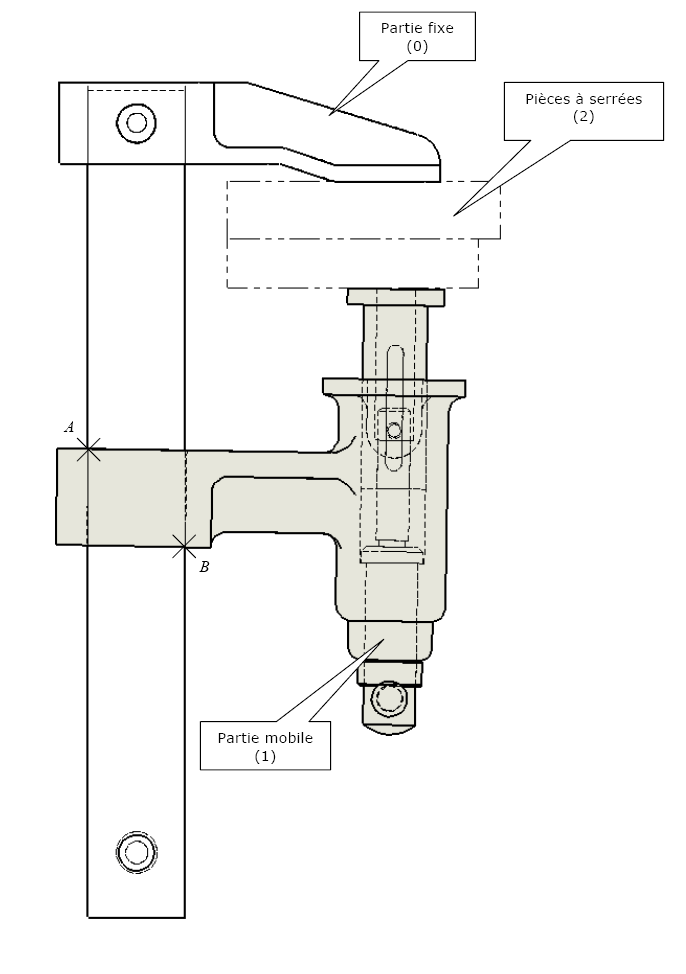
\includegraphics[width=0.8\linewidth]{img/serre-joint_graph.png}
\end{figure}

\ifdef{\public}{\end{document}}{}

\newpage

\section{Correction}

\subsection{Mandrin à serrage pneumatique}

\paragraph{Question 1:}

$X_f=P.S=30.0,1.\pi.\frac{157^2-45^2}{4}=53300$

\paragraph{Question 2:}

$\left\{T_{i\rightarrow 4}\right\}=\left\{\begin{array}{cc}
X_{i4} & 0 \\ 0 & M_{i4} \\  0 & N_{i4}
\end{array}\right\}_{A_i,R'_i}=\left\{\begin{array}{cc}
cos\alpha.X_{i4} & -sin\alpha.M_{i4} \\ sin\alpha.X_{i4} & cos\alpha.M_{i4} \\  0 & N_{i4}
\end{array}\right\}_{A_i,R_i}$

$\left\{T_{i\rightarrow 4}\right\}=\left\{\begin{array}{cc}
cos\alpha.X_{i4} & -sin\alpha.M_{i4} \\ sin\alpha.X_{i4} & cos\alpha.M_{i4} \\  0 & N_{i4}-e.cos\alpha.X_{i4}
\end{array}\right\}_{O_0,R_i}$

\paragraph{Question 3:}

$\left\{T_{i\rightarrow 4}\right\}=\left\{\begin{array}{cc}
cos\alpha.X_{i4} & -sin\alpha.M_{i4} \\ sin\alpha.X_{i4}.cos\beta_i & cos\alpha.M_{i4}.cos\beta_i-(N_{i4}-e.cos\alpha.X_{i4}).sin\beta_i \\ sin\alpha.X_{i4}.sin\beta_i & cos\alpha.M_{i4}.sin\beta_i+(N_{i4}-e.cos\alpha.X_{i4}).cos\beta_i
\end{array}\right\}_{O_0,R_0}$

Or, $\left\{\begin{array}{l}
X_{14}=X_{24}=X_{34}=X_{i4} \\
M_{14}=M_{24}=M_{34}=M_{i4} \\
cos0+cos\frac{2.\pi}{3}+cos\frac{4.\pi}{3}=0 \\
sin0+sin\frac{2.\pi}{3}+sin\frac{4.\pi}{3}=0
\end{array}\right.$

Donc, 

$\left\{T_{\sum Mors \rightarrow S_4}\right\}=\left\{
  \begin{array}{c c}
  X_{\sum Mors \rightarrow S_4} & L_{\sum Mors \rightarrow S_4} \\
  0 & 0 \\
  0 & 0
  \end{array}\right\}_{O,R_0}$

\paragraph{Question 4:}

Or, $\left\{\begin{array}{l}
X_{\sum Mors \rightarrow S_4}=3.cos\alpha.X_{i4} \\
L_{\sum Mors \rightarrow S_4}=-3.sin\alpha.M_{i4}
\end{array}\right.$

\paragraph{Question 5:}

$\left\{T_{0\rightarrow 4}\right\}=\left\{\begin{array}{cc}
0 & 0 \\ Y_{04} & M_{04} \\ Z_{04} & N_{04}
\end{array}\right\}_{O_0,R_0}$

\paragraph{Question 6:}

$\left\{\begin{array}{l}
X_f+3.cos\alpha.X_{i4}=0 \\
Y_{04}=0 \\
Z_{04}=0 \\
-3.sin\alpha.M_{i4}=0 \\
M_{04}=0 \\
N_{04}=0 \\
\end{array}\right.$

\paragraph{Question 7:}

$\left\{T_{0\rightarrow 4}\right\}=\left\{0\right\}$

\paragraph{Question 8:}

$\left\{\begin{array}{l}
X_{14}=-\frac{X_f}{3.cos\alpha} \\
M_{14}=0
\end{array}\right.$

\paragraph{Question 9:}

$\left\{T_{0\rightarrow 1}\right\}=\left\{\begin{array}{cc}
X_{01} & L_{01} \\ 0 & M_{01} \\ Z_{01} & N_{01}
\end{array}\right\}_{O_0,R_0}$

$\left\{T_{4\rightarrow 1}\right\}=\left\{\begin{array}{cc}
-X_{14}.cos\alpha & 0 \\ -X_{14}.sin\alpha & 0 \\ 0 & -N_{14}+e.cos\alpha.X_{14}
\end{array}\right\}_{O_0,R_0}$

$\left\{T_{5\rightarrow 1}\right\}=\left\{\begin{array}{cc}
X_{51} & R.Z_{51} \\ Y_{51} & 0 \\ Z_{51} & -R.X_{51}
\end{array}\right\}_{O_0,R_0}$

\paragraph{Question 10:}

$\left\{\begin{array}{l}
X_{01}-X_{14}.cos\alpha+X_{51}=0 \\
-X_{14}.sin\alpha+Y_{51}=0 \\
Z_{01}+Z_{51}=0 \\
L_{01}+R.Z_{51}=0 \\
M_{01}=0 \\
N_{01}-N_{14}+e.cos\alpha.X_{14}-R.X_{51}=0
\end{array}\right.$

\paragraph{Question 11:}

$Y_{51}=-\dfrac{tan 30}{3}.53305\approx -10000N\approx -10000daN$

\paragraph{Question 12:}

$|Y_{5\rightarrow 1}|=-10000daN>-500daN$

\paragraph{Question 13:}

$Z_{51}<f.Y_{51}$

$C_{s}<3.Z_{51max}.R$

$C_{s}<3.0,3.10000.10.10^{-3}=90N.m$

\subsection{Serre joint}

\begin{center}
 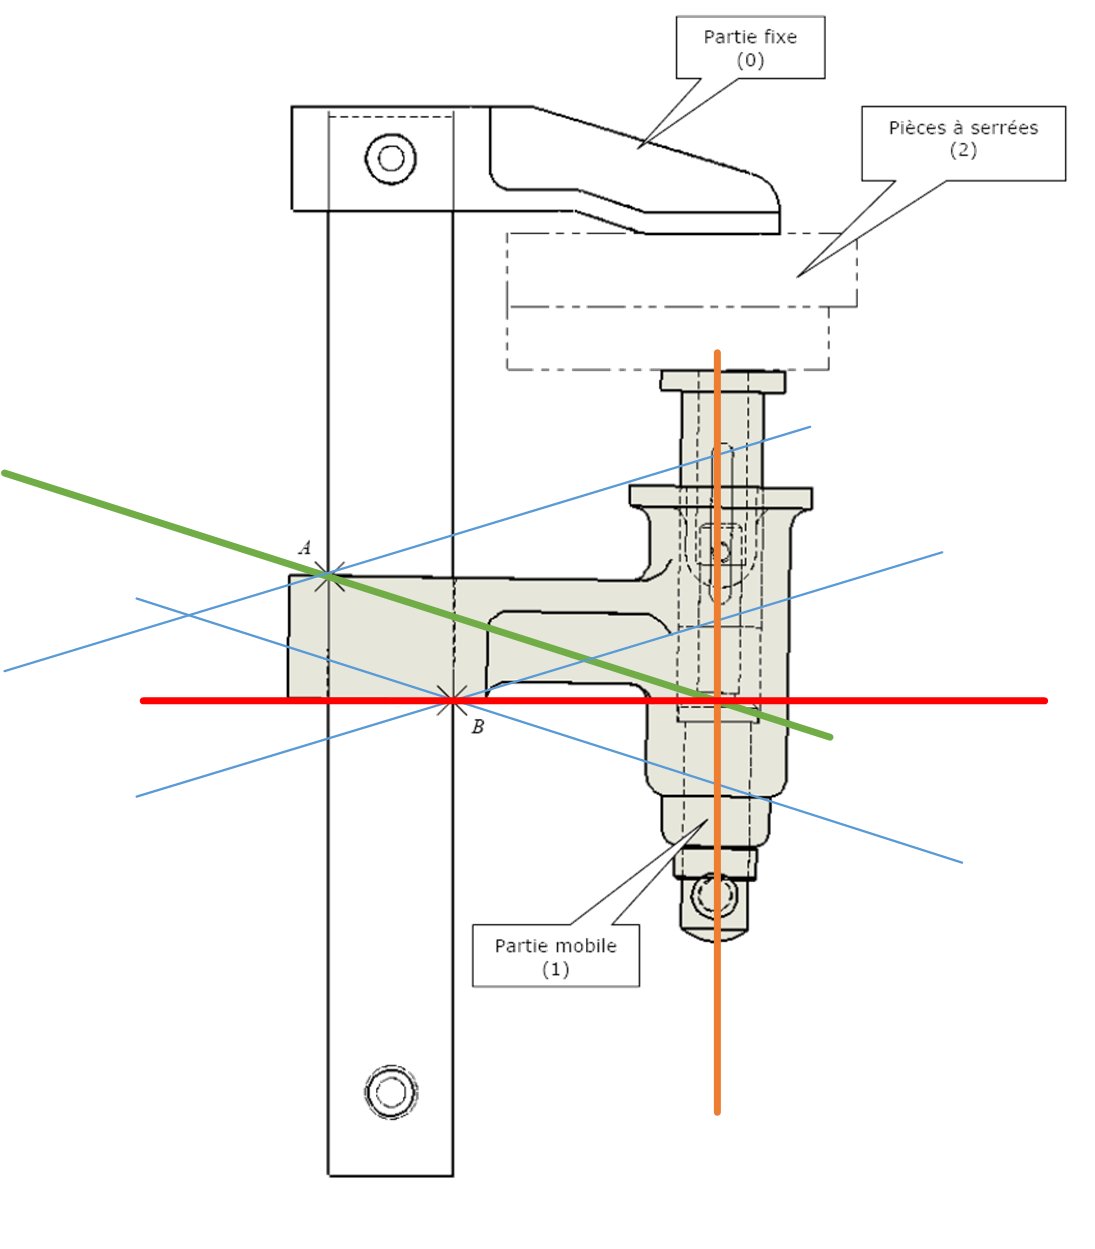
\includegraphics[width=0.8\linewidth]{img/graph_cor}
\end{center}
\end{document}
